% modeling conditional distributions
\documentclass[../main.tex]{subfiles}
\begin{document}
	
	\textbf{Modeling for and estimation of the distributions of potential outcomes}\\
	Under the conditions of Lemma 1, we can solve Problem (2) under a sequence of $\mu$ converging to zero, and the solution $\underset{\mu \to 0}{\lim} \bs{\tau}_{\kappa}^*(\mu) = \bs{\tau}_{\kappa}^0$. However, as the distribution of potential outcomes are unknown, the two major quantities under an arbitrary regime $\bs{d}$ involved, $\mb{E}Y^*(\bs{d})$ and $\mb{E}Z^*(\bs{d})$, need to be estimated from the observed data. Our strategy for estimating these two quantities is to model the marginal distribution of each potential outcome, and then draw Monte-Carlo random samples from the estimated marginal distributions to calculate their expectations numerically.\\
	

	To connect  observed data with potential outcomes, three necessary causal inference assumptions are needed. \\
	\begin{enumerate}
		\item Consistency: $Y = Y^*(A_1, A_2)$.
		\item Sequential ignorability: $A_t  \indep W^*  | \bs{H}_{t}$ for $t =1 ,2$.
		\item Positivity: $\exists \epsilon > 0$ for which $\epsilon < \text{Pr}(A_t = a_t \mid \bs{H}_t) < 1 - \epsilon$ with probabilty one for all $a_t$, $t=1, 2$.
	\end{enumerate}
	Following the G-computation formula by Robins etc.~\cite{Gill2001}, we have, for any arbitrary regime $\bs{d} = (d_1, d_2) $, that
	\begin{flalign*}	
	\text{Pr}\{ Y^*(\bs{d}) \le y\} = \mb{E}_{\bs{X}_1} \lt\{ \mb{E}_{\bs{X}_2}\lt[  \text{Pr}\lt\{Y \le y \mid \bs{X}_2 , A_2 = d_2(\bs{X}_2), \bs{X}_1 , A_1 = d_1(\bs{X}_1)\rt\}  \mid \bs{X}_1, A_1 = d_1(\bs{X}_1) \rt] \rt\}
	\end{flalign*}
	
	%\begin{equation*}	\
	%\text{Pr}\{ Y^*(\bs{d}) > y\} =\mb{E} \left[ \underset{a_1}{\sum} \mathds{1}_{a_1 = d_1(\bs{H}_1)} \mb{E}\left\{ \underset{a_2}{\sum} \mathds{1}_{a_2 = d_2(\bs{H}_2)} \text{Pr} (Y > y \rvert \bs{X}_1 = \bs{x}_1, A_1 = a_1, \bs{X}_2 = \bs{x}_2, A_2=a_2)  \mid \bs{X}_1, A_1 = a_1\right\}\right],
	%\end{equation*}
	and similarly, 
	\begin{flalign*}	
	\text{Pr}\{ Z^*(\bs{d}) \le z\} =  \mb{E}_{\bs{X}_1} \lt\{ \mb{E}_{\bs{X}_2}\lt[  \text{Pr}\lt\{Z \le z \mid \bs{X}_2 , A_2 = d_2(\bs{X}_2), \bs{X}_1 , A_1 = d_1(\bs{X}_1)\rt\}  \mid \bs{X}_1, A_1 = d_1(\bs{X}_1) \rt] \rt\}
	\end{flalign*}
	
	%	\begin{gather*}
	%	\begin{flalign*}
	%	& \text{Pr}\{ Z^*(\bs{d}) > z\} =\\
	%	& \mb{E} \left[ \underset{a_1}{\sum} \mathds{1}_{a_1 = d_1(\bs{H}_1)} \mb{E}\left\{ \underset{a_2}{\sum} \mathds{1}_{a_2 = d_2(\bs{H}_2)} \text{Pr} (Z > z \rvert \bs{X}_1 = \bs{x}_1, A_1 = a_1, \bs{X}_2 = \bs{x}_2, A_2=a_2) \rvert \bs{X}_1, A_1 = a_1\right\}\right].
	%	\end{flalign*}
	%	\end{gather*}
	
	%\begin{flalign*}
	%& \text{Pr}\{ Y^*(\bs{d}) > y\} =\\
	%& \mb{E} \left[ \underset{a_1}{\sum} \mathds{1}_{a_1 = d_1(\bs{H}_1)} \mb{E}\left\{ \underset{a_2}{\sum} \mathds{1}_{a_2 = d_2(\bs{H}_2)} \text{Pr} (Y > y \rvert \bs{H}_2, A_2)  \mid \bs{H}_1, A_1 \right\}\right],
	%\end{flalign*}
	
	%\marginnote{\small{Review G-computation!}}[-1.5cm]
	%\begin{flalign*}
	%& \text{Pr}\{ Z^*(\bs{d}) > z\} =\\
	%& \mb{E} \left[ \underset{a_1}{\sum} \mathds{1}_{a_1 = d_1(\bs{H}_1)} \mb{E}\left\{ \underset{a_2}{\sum} \mathds{1}_{a_2 = d_2(\bs{H}_2)} \text{Pr} (Z > z \rvert \bs{H}_2 , A_2 ) \mid \bs{H}_1 , A_1 \right\}\right].
	%\end{flalign*}
	
	Hence, we can estimate the probabilty function of the potential outcomes under a regime $\bs{d}$, $\text{Pr}\{ Y^*(\bs{d}) \le y\}$ and $\text{Pr}\{ Z^*(\bs{d}) \le z\}$  , using observed data by modeling and estimating the conditional distributions involved, and hence, $\mb{E}Y^*(\bs{d})$ and $\mb{E}Z^*(\bs{d})$.\\
	 
For now, we follow the modeling tactic in Interactive Q-learning for Quantiles by Linn et al. We assume the following model, 
\begin{flalign*}
& Y  = \mb{E}(Y \rvert \bs{H}_2, A_2)  + \varepsilon_Y,  \\
& \mb{E}(Y \rvert \bs{H}_2, A_2)  = m_Y(\bs{H}_2) + A_2 c_Y(\bs{H}_2), \\
& \text{where } \mb{E}(\varepsilon_Y) = 0, \text{Var}(\varepsilon_Y) = \sigma^2, \text{and } \varepsilon_Y \indep (\bs{H}_2, A_2).
\end{flalign*}

Define $F_{\varepsilon_Y}(\cdot)$ to be the distribution of $\varepsilon_Y$; $F_{\bs{H}_2 \rvert \bs{H}_1, A_1}(\cdot \mid \bs{h}_1, a_1)$ to be the conditional distribution of $\bs{H}_2$ given $\bs{H}_1 = \bs{h}_1$ and $A_1 = a_1$; $F_{\bs{H}_1}(\cdot)$ to be the distribution of $\bs{H}_1$. Again, we have $\bs{H}_1^\itl = (1, \bs{X}^\itl_1)$, $d_1(\bs{H}_1)$, $\bs{H}_2 = \{ \bs{H}^\itl_1, d_1(\bs{H}_1), \bs{X}^\itl_2\}^\itl$. \\	
%	Let $J^{d_1, d_2}(\bs{h}_1, \bs{h}_2, y) = F_{\varepsilon_Y}\{ y - m(\bs{h_2}^{d_1(\bs{h_1})}) - d_2(\bs{h}_2^{d_1(\bs{h}_1)})c_Y(\bs{h}_2^{d_1(\bs{h}_1)}) \}$, then
\begin{flalign*}
& \text{Pr}^{\bs{d}}\lt\{ Y \le y \mid \bs{H}_2 =\bs{h}_2, d_2(\bs{H}_2) =d_2(\bs{h}_2) \rt\} \\
= & \text{Pr}^{\bs{d}}\lt\{ m(\bs{H}_2 )+ d_2( \bs{H}_2)c_Y(\bs{H}_2) + \varepsilon_Y \le y \mid \bs{H}_2 =\bs{h}_2, d_2(\bs{H}_2) =d_2(\bs{h}_2)  \rt\} \\
= & \text{Pr}^{\bs{d}}\lt\{ \varepsilon_Y \le y - m(\bs{H}_2) - d_2( \bs{H}_2)c_Y(\bs{H}_2) \mid \bs{H}_2 =\bs{h}_2, d_2(\bs{H}_2) =d_2(\bs{h}_2) \rt\}\\
=&  F_{\varepsilon_Y}\lt\{ y - m(\bs{h}_2) - d_2(\bs{h}_2)c_Y(\bs{h}_2) \rt\}\\
= &  F_{\varepsilon_Y}\lt[ y - m(\bs{h}_2) - \tsgn\lt\{r_2(\bs{h}_2; \bs{\tau}_2)\rt\}c_Y(\bs{h}_2) \rt]
\end{flalign*}
Hence, we have
\begin{flalign*}
& \text{Pr}\lt\{ Y^*({\bs{d}}) \le y  \rt\} \\  
= &  \iint \text{Pr}^{\bs{d}}\lt\{ Y \le y \mid  \bs{H}_2=\bs{h}_2, d_2(\bs{H}_2)= d_2(\bs{h}_2) \rt\} \,d F_{\bs{H}_2 \mid \bs{H}_1, A_1}\lt\{ \bs{h}_2 \rvert d_1(\bs{\bs{h}_1}), \bs{h}_1 \rt\} \,d F_{\bs{H}_1}(\bs{h}_1)\\
= &  \iint  F_{\varepsilon_Y}\lt\{ y - m(\bs{h}_2) - d_2(\bs{h}_2)c_Y(\bs{h}_2) \rt\} \,d F_{\bs{H}_2 \mid  \bs{H}_1, A_1}\lt\{ \bs{h}_2 \mid \bs{h}_1 , d_1(\bs{h}_1)\rt\} \,d F_{\bs{H}_1}(\bs{h}_1)\\
% = & \iint  F_{\varepsilon_Y}\lt\{ y - m_Y(\bs{h}_2) - d_2(\bs{h}_2)c_Y(\bs{h}_2) \rt\} \,d G_{Y}\lt\{ m_Y, c_Y \rvert \bs{h}_1 , d_1(\bs{h}_1)\rt\} \,d F_{\bs{H}_1}(\bs{h}_1) \\
= &  \iint  F_{\varepsilon_Y}\lt[ y - m(\bs{h}_2) - \tsgn\lt\{r_2(\bs{h}_2; \bs{\tau}_2)\rt\}c_Y(\bs{h}_2) \rt] \,d G_{Y}\lt\{ m_Y, c_Y, r_2 \rvert \bs{h}_1 , d_1(\bs{h}_1)\rt\} \,d F_{\bs{H}_1}(\bs{h}_1) \\
= &  \iint  F_{\varepsilon_Y}\lt[ y - m(\bs{h}_2) - \tsgn(r_2)c_Y(\bs{h}_2) \rt] \,d G_{Y}\lt\{ m_Y, c_Y, r_2 \rvert \bs{h}_1 , d_1(\bs{h}_1)\rt\} \,d F_{\bs{H}_1}(\bs{h}_1) 
\end{flalign*}
where $G_{Y}\lt\{ m_Y , c_Y, r_2\mid \bs{h}_1, a_1 \rt\}$ is the joint conditional distribution of $m_Y\lt(\bs{H}_2\rt)$, $c_Y\lt(\bs{H}_2\rt)$ and $r_2(\bs{H}_2; \bs{\tau}_2)$ given $\bs{H}_1 = \bs{h}_1$ and $A_1 = a_1$. The second equality is due to  $\int z(x, y) \,d F_{X | Y}(x | y) = \mb{E}(z | y) = \int z\,d F_{Z | Y}(z | y).$\\
w
Same applies to $Z$:
\begin{flalign*}
& Z  = \mb{E}(Z \rvert \bs{H}_2, A_2)  + \epsilon, \\
& \text{where } \mb{E}(\epsilon) = 0, \text{Var}(\epsilon) = \sigma^2, \text{and } \epsilon \indep (\bs{H}_2, A_2) \\
& \mb{E}(Z \rvert \bs{H}_2, A_2)  = m_Z(\bs{H}_2) + A_2 c_Z(\bs{H}_2)
\end{flalign*}
\begin{flalign*}
& \text{Pr}\lt\{ Z^*({\bs{d}}) \le z  \rt\} \\  
= &  \iint \text{Pr}^{\bs{d}}\lt\{ Z \le z \mid  \bs{H}_2=\bs{h}_2, d_2(\bs{H}_2)= d_2(\bs{h}_2) \rt\} \,d F_{\bs{H}_2 \mid \bs{H}_1, A_1}\lt\{ \bs{h}_2 \rvert d_1(\bs{\bs{h}_1}), \bs{h}_1 \rt\} \,d F_{\bs{H}_1}(\bs{h}_1)\\
= &  \iint  F_{\varepsilon_Z}\lt\{ z - m(\bs{h}_2) - d_2(\bs{h}_2)c_Z(\bs{h}_2) \rt\} \,d F_{\bs{H}_2 \mid  \bs{H}_1, A_1}\lt\{ \bs{h}_2 \mid \bs{h}_1 , d_1(\bs{h}_1)\rt\} \,d F_{\bs{H}_1}(\bs{h}_1)\\
% = & \iint  F_{\varepsilon_Z}\lt\{ z - m_Z(\bs{h}_2) - d_2(\bs{h}_2)c_Z(\bs{h}_2) \rt\} \,d G_{Z}\lt\{ m_Z, c_Z \rvert \bs{h}_1 , d_1(\bs{h}_1)\rt\} \,d F_{\bs{H}_1}(\bs{h}_1) \\
= &  \iint  F_{\varepsilon_Z}\lt[ z - m(\bs{h}_2) - \tsgn\lt\{r_2(\bs{h}_2; \bs{\tau}_2)\rt\}c_Z(\bs{h}_2) \rt] \,d G_{Z}\lt\{ m_Z, c_Z, r_2 \rvert \bs{h}_1 , d_1(\bs{h}_1)\rt\} \,d F_{\bs{H}_1}(\bs{h}_1) \\
= &  \iint  F_{\varepsilon_Z}\lt[ z - m(\bs{h}_2) - \tsgn(r_2)c_Z(\bs{h}_2) \rt] \,d G_{Z}\lt\{ m_Z, c_Z, r_2 \rvert \bs{h}_1 , d_1(\bs{h}_1)\rt\} \,d F_{\bs{H}_1}(\bs{h}_1) 
\end{flalign*}

where $G_{Z}\lt\{ m_Z, c_Z, r_2 \mid \bs{h}_1, a_1 \rt\}$ is the joint conditional distribution of $m_Z\lt(\bs{H}_2\rt)$, $c_Z\lt(\bs{H}_2\rt)$ and $r_2(\bs{H}_2; \bs{\tau}_2)$ given $\bs{H}_1 = \bs{h}_1$ and $A_1 = a_1$. \\

Details of estimation and modeling follows ``Estimation of dynamic treatment regimes for complex outcomes: Balancing benefits and risks" by Linn et al.\\

\textbf{Estimation of the barrier trajectory} \\
Once we have the estimators of $\mb{E}Y^*(\bs{\tau})$ and $\mb{E}Z^*(\bs{\tau})$, denoted by $\wh{\mb{E}}Y_n(\bs{\tau})$ and $\wh{\mb{E}}Z_n(\bs{\tau})$, we plug  those estimators into Problem (2), and get Problem (3) as
\begin{equation}
\underset{\bs{\tau}}{\max }\,\, \wh{\mb{E}} Y_n(\bs{\tau}) + \mu \txt{log} \lt\{ \kappa - \wh{\mb{E}} Z_n(\bs{\tau}) \rt\} - \frac{1}{2\mu} \lt\{ (\bs{\tau}_1^\itl \bs{\tau}_1 -1 )^2 + (\bs{\tau}_2^\itl \bs{\tau}_2 -1 )^2 \rt\}
\end{equation}
 Denote a solution to Problem (3) by $\wh{\bs{\tau}}_{\kappa}(\mu) = (\wh{\bs{\tau}}^\itl_{\kappa,\mu,1} , \wh{\bs{\tau}}_{\kappa,\mu,2}^\itl )^\itl$, and $\widehat{S}(\bs{\tau}, \mu) = \wh{\mb{E}} Y_n(\bs{\tau}) + \mu \, \txt{log} \lt\{ \kappa - \wh{\mb{E}}Z_n(\bs{\tau}) \rt\} - \frac{1}{2\mu} \lt\{ (\bs{\tau}_1^\itl \bs{\tau}_1 -1 )^2 + (\bs{\tau}_2^\itl \bs{\tau}_2 -1 )^2 \rt\}.$ The following figure is an replication of the simulation result in the ``Estimation of dynamic treatment regimes for complex outcomes" chapter.\\

 
\begin{overpic}[width=0.90\textwidth]{test7}
	\put (0, 57) {$\wh{\mb{E} }Y_n(\wh{\bs{\tau}}_{\kappa,\mu})$}
	\put (0, 27) {$\wh{\mb{E} }Z_n(\wh{\bs{\tau}}_{\kappa,\mu})$}
	\put (50, 2.5) {$\kappa$}
\end{overpic}
%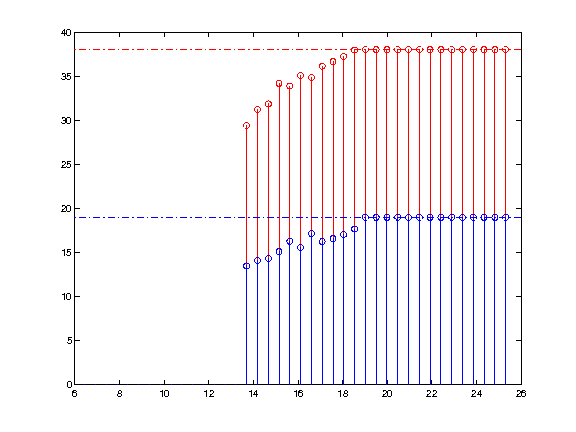
\includegraphics{test7}

The red bars are  the estimated means of $Y$ under the  estimated constrained optimal regimes vs. constraint value $\kappa$. The blue bars are  the estimated means of $Z$ under the estimated constrained optimal regime vs. constrain value $\kappa$. The red dash line is the estimated maximal of $Y$ without constraint, and the blue dash line is the estimated minimal of $Z$ without constraint. For the constrained problems, Matlab fmincon  solver is used with `Algorithm' option set to `interior-point' method, and `FinDiffRelStep' to 1e-2.  For unconstrained problems, Matlab fminunc solver is used,where `Algorithm' options is set to `quasi-newton', and `FinDiffRelStep' to 1e-2. MultiStart function is called for 5 random starts, where `StartPointsToRun' option is set to `all'. 
\end{document}